%!TEX root = ../main.tex

\section{Results}
\label{section:cfgnn-results}


We evaluate CF-GNNExplainer in terms of the metrics outlined in Section~\ref{section:cfgnn-metrics}. 
The results are shown in Table~\ref{table:results1} and Table~\ref{table:results-gnnexplainer}.  
In cases where the baselines outperform CF-GNNExplainer on a particular metric, they perform poorly on the rest of the metrics, or on other datasets. 




\subsection{Main Findings}

\textbf{Fidelity:}
CF-GNNExplainer outperforms \basekeep{} across all three datasets, and outperforms \baserm{} for \synfour{} and \synfive{} in terms of fidelity. 
We find that \baserand{} has the lowest fidelity in all cases -- it is able to find counterfactual examples for every single node. 
In the following subsections, we will see that this corresponds to poor performance on the other metrics.

\begin{table*}[h]
\centering
\caption{Results comparing our method (abbreviated as \OurShort{}) to \baserand{}, \basekeep{}, and \baserm{}. Below each metric, $\blacktriangledown$ indicates a low value is desirable, while $\blacktriangle$ indicates a high value is desirable.}
\label{table:results1}
\setlength{\tabcolsep}{4pt}
\scriptsize{
\begin{tabular}{lrrrr rrrr rrrr}
\toprule
\multicolumn{1}{c}{} & \multicolumn{4}{c}{\synfour{}}                                                                                                                 & \multicolumn{4}{c}{\synfive{}}                                                                                                                   & \multicolumn{4}{c}{\synone{}}                                                                                                                  \\ 
\cmidrule(r){2-5}\cmidrule(r){6-9}\cmidrule{10-13} 
               & \multicolumn{1}{c}{Fid.} & \multicolumn{1}{c}{Size} & \multicolumn{1}{c}{Spar.} & \multicolumn{1}{c}{Acc.} & \multicolumn{1}{c}{Fid.} & \multicolumn{1}{c}{Size} & \multicolumn{1}{c}{Spar.} & \multicolumn{1}{c}{Acc.} & \multicolumn{1}{c}{Fid.} & \multicolumn{1}{c}{Size} & \multicolumn{1}{c}{Spar.} & \multicolumn{1}{c}{Acc.} \\

% & \multicolumn{1}{c}{$\downarrow$} &\multicolumn{1}{c}{$\downarrow$} &\multicolumn{1}{c}{$\uparrow$} & \multicolumn{1}{c}{$\uparrow$} & \multicolumn{1}{c}{$\downarrow$} &\multicolumn{1}{c}{$\downarrow$} &\multicolumn{1}{c}{$\uparrow$} & \multicolumn{1}{c}{$\uparrow$} & \multicolumn{1}{c}{$\downarrow$} &\multicolumn{1}{c}{$\downarrow$} &\multicolumn{1}{c}{$\uparrow$} & \multicolumn{1}{c}{$\uparrow$} \\

Method & \multicolumn{1}{c}{$\blacktriangledown$} &\multicolumn{1}{c}{$\blacktriangledown$} &\multicolumn{1}{c}{$\blacktriangle$} & \multicolumn{1}{c}{$\blacktriangle$} & \multicolumn{1}{c}{$\blacktriangledown$} &\multicolumn{1}{c}{$\blacktriangledown$} &\multicolumn{1}{c}{$\blacktriangle$} & \multicolumn{1}{c}{$\blacktriangle$} & \multicolumn{1}{c}{$\blacktriangledown$} &\multicolumn{1}{c}{$\blacktriangledown$} &\multicolumn{1}{c}{$\blacktriangle$} & \multicolumn{1}{c}{$\blacktriangle$} \\
\midrule
\baserand{}               & \textbf{0.00}                     & 4.70                              & 0.79                                & 0.63                               & \textbf{0.00}                     & 9.06                              & 0.75                                & 0.77                               & \textbf{0.00}                     & 503.31                            & 0.58                                & 0.17                              \\
\basekeep{}                 & 0.32                              & 15.64                             & 0.13                                & 0.45                               & 0.32                              & 29.30                             & 0.09                                & 0.72                               & 0.60                              & 504.18                            & 0.05                                & 0.18                              \\
\baserm{}              & 0.46                              & 2.11                              & 0.89                                & ---                                  & 0.61                              & 2.27                              & 0.92                                & ---                                  & 0.21                              & 10.56                             & 0.97                                & \textbf{0.99}                     \\


% \gnnexpshort{} ($S=$ GT) &  0.55 &	6.00 & 0.57 &	0.46 &	0.35 &	11.83 &	0.53 &	0.74 &	0.82 &	6.00 &	0.79 &	0.24    \\

\midrule
CF-GNN              & 0.21                              & \textbf{2.09}                     & \textbf{0.90}                       & \textbf{0.94}                      & 0.07                              & \textbf{1.47}                     & \textbf{0.94}                       & \textbf{0.96}                      & 0.39                              & \textbf{2.39}                     & \textbf{0.99}                       & 0.96                 \\
\bottomrule
\end{tabular}
}
\end{table*}





\medskip \noindent
\textbf{Explanation Size:}
Figures~\ref{fig:random-explanation-size} to~\ref{fig:explanation-size} show histograms of the explanation size for CF-GNNExplainer and the baselines. 
We see that across all three datasets, CF-GNNExplainer has the smallest (i.e., most minimal) explanation sizes. 
This is especially true when comparing to \baserand{} and \basekeep{} for the \synone{} dataset, where we had to use a different scale for the $x$-axis due to how different the explanation sizes were. 
We postulate that this difference could be because \synone{} is a much more densely connected graph;
it has fewer nodes but more edges compared to the other two datasets, and the average number of nodes and edges in the \cgraph{} is order(s) of magnitude larger (see Table~\ref{table:stats}). 
Therefore, when performing random perturbations, there is substantial opportunity to remove edges that do not necessarily need to be removed, leading to much larger explanation sizes.
When there are many edges in the \cgraph{}, removing everything except the 1-hop neighbourhood, as is done in \basekeep{}, also results in large explanation sizes. 
In contrast, the loss function used by CF-GNNExplainer ensures that only a few edges are removed, which is the desirable behavior since we want minimal explanations. 

\pagebreak

\medskip \noindent
\textbf{Sparsity:}
CF-GNNExplainer outperforms the \baserand{}, \baserm{}, \basekeep{} baselines for all three datasets in terms of sparsity.
%\footnote{GNNExplainer cannot be evaluated on sparsity.} 
We note CF-GNNExplainer and \baserm{} perform much better on this metric in comparison to the other methods, which aligns with the results from explanation size. 

\medskip \noindent
\textbf{Accuracy:}
We observe that CF-GNNExplainer has the highest accuracy for the \synfour{} and \synfive{} datasets, whereas \baserm{} has the highest accuracy for \synone{}. 
However, we are unable to calculate the accuracy of \baserm{} for the other two datasets since it is unable to generate \emph{any} counterfactual examples for motif nodes, contributing to the low sparsity on those datasets. 
We observe accuracy levels upwards of 94\% for CF-GNNExplainer across \emph{all} datasets, indicating that it is consistent in correctly removing edges that are crucial for the initial predictions in the vast majority of cases (see Table~\ref{table:results1}). 






\begin{figure*}[]

    \centering

    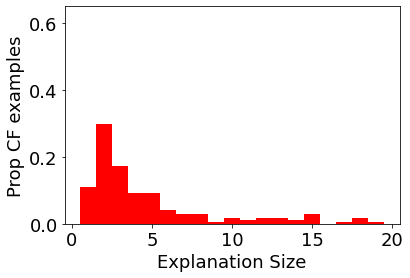
\includegraphics[scale=0.27]{04-research-cfgnn/images/tree-cycles-random.png}
    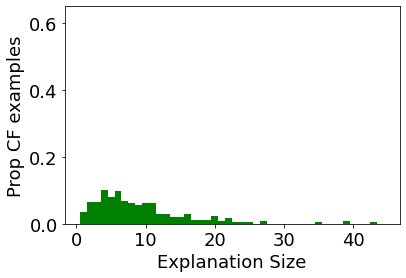
\includegraphics[scale=0.27]{04-research-cfgnn/images/tree-grid-random.png}
    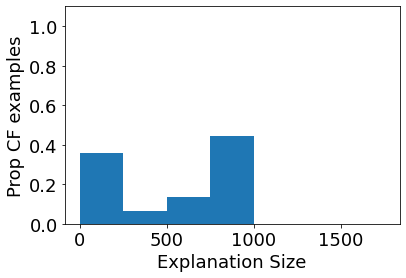
\includegraphics[scale=0.27]{04-research-cfgnn/images/ba-shapes-random.png}
    
        \caption{Histograms showing the proportion of counterfactual examples that have a certain explanation size from \baserand{}. Note the $x$-axis for \synone{} goes up to 1500. Left: \synfour{}, Middle: \synfive{}, Right: \synone{}.  }
        \label{fig:random-explanation-size}
        \bigskip \bigskip
        
    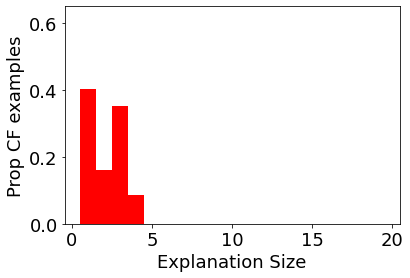
\includegraphics[scale=0.27]{04-research-cfgnn/images/tree-cycles-keep.png}
    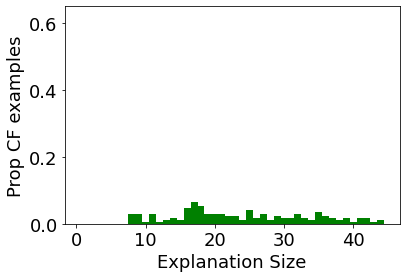
\includegraphics[scale=0.27]{04-research-cfgnn/images/tree-grid-keep.png}
    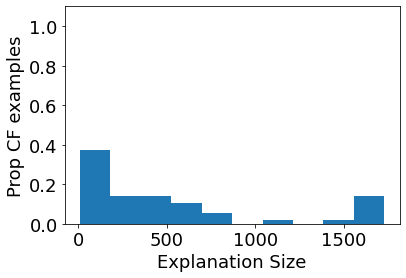
\includegraphics[scale=0.27]{04-research-cfgnn/images/ba-shapes-keep.png}
    
        \caption{Histograms showing the proportion of counterfactual examples that have a certain explanation size from \basekeep{}. Note the $x$-axis for \synone{} goes up to 1500. Left: \synfour{}, Middle: \synfive{}, Right: \synone{}. }
        \label{fig:keep-explanation-size}
        \bigskip \bigskip
        
        
    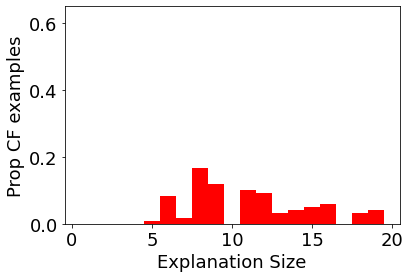
\includegraphics[scale=0.27]{04-research-cfgnn/images/tree-cycles-remove.png}
    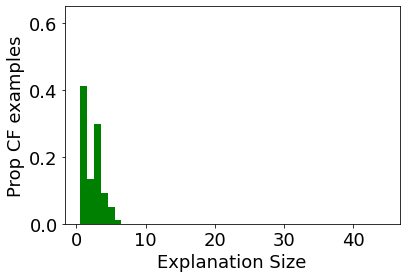
\includegraphics[scale=0.27]{04-research-cfgnn/images/tree-grid-remove.png}
    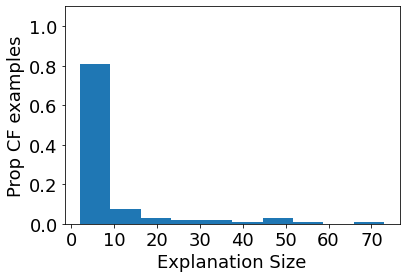
\includegraphics[scale=0.27]{04-research-cfgnn/images/ba-shapes-remove.png}
    
        \caption{Histograms showing the proportion of counterfactual examples that have a certain explanation size from \baserm{}. Note the $x$-axis for \synone{} goes up to 70. Left: \synfour{}, Middle: \synfive{}, Right: \synone{}. }
        \label{fig:remove-explanation-size}
        \bigskip \bigskip
        
    % 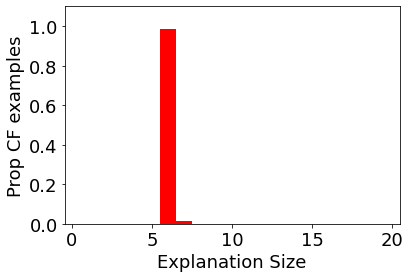
\includegraphics[scale=0.38]{images/tree-cycles-gnnexplainer.png}
    % 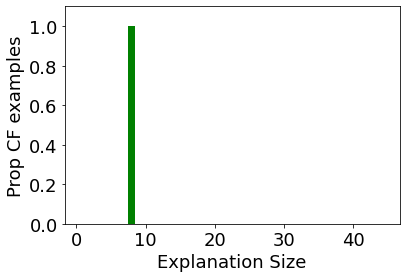
\includegraphics[scale=0.38]{images/tree-grid-gnnexplainer.png}
    % 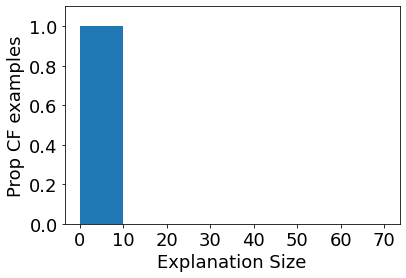
\includegraphics[scale=0.38]{images/ba-shapes-gnnexplainer.png}
    
    %     \caption{Histograms showing explanation size from \gnnexplainer{} for $S=$ GT. Note that the y-axis goes up to 1. Left: \synfour{}, Middle: \synfive{}, Right: \synone{}.}
    %     \label{fig:gnnexplainer-explanation-size}

    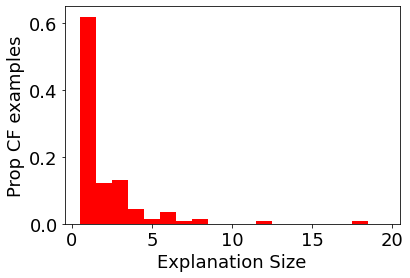
\includegraphics[scale=0.27]{04-research-cfgnn/images/tree-cycles.png}
    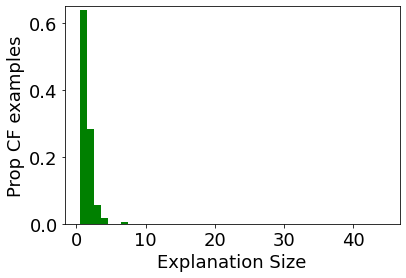
\includegraphics[scale=0.27]{04-research-cfgnn/images/tree-grid.png}
    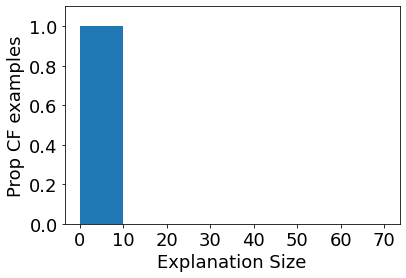
\includegraphics[scale=0.27]{04-research-cfgnn/images/ba-shapes.png}
    
        \caption{Histograms showing the proportion of counterfactual examples that have a certain explanation size from CF-GNNExplainer. Note the $x$-axis for \synone{} goes up to 70. Left: \synfour{}, Middle: \synfive{}, Right: \synone{}. }
        \label{fig:explanation-size}
        
\end{figure*}







\subsection{Comparison to \gnnexplainer{}}
Table~\ref{table:results-gnnexplainer} shows the results comparing our method to \gnnexplainer{}. We find that our method outperforms \gnnexplainer{} across all three datasets in terms of both fidelity and accuracy, for all tested values of $S$. 
However, this is not surprising since \gnnexplainer{} is not meant for generating counterfactual explanations, so we cannot expect it to perform well on a task it was not designed for. 
We cannot compare explanation size or sparsity fairly since \gnnexplainer{} requires the user to input the value of $S$. 



\begin{table*}[]
\centering
\caption{Results comparing our method to \gnnexplainer{}. \gnnexplainer{} cannot find $S$ automatically, so we try varying values of $S$. GT indicates the size of the ground truth explanation for each dataset. CF-GNNExplainer finds $S$ automatically. Below each metric, $\blacktriangledown$ indicates a low value is desirable, while $\blacktriangle$ indicates a high value is desirable.}
\label{table:results-gnnexplainer}
\setlength{\tabcolsep}{4pt}
\scriptsize{
\begin{tabular}{lrrrr rrrr rrrr}
\toprule
\multicolumn{1}{c}{} & \multicolumn{4}{c}{\synfour{}}                                                                                                                 & \multicolumn{4}{c}{\synfive{}}                                                                                                                   & \multicolumn{4}{c}{\synone{}}                                                                                                                  \\ 
\cmidrule(r){2-5}\cmidrule(r){6-9}\cmidrule{10-13} 
               & \multicolumn{1}{c}{Fid.} & \multicolumn{1}{c}{Size} & \multicolumn{1}{c}{Spars.} & \multicolumn{1}{c}{Acc.} & \multicolumn{1}{c}{Fid.} & \multicolumn{1}{c}{Size} & \multicolumn{1}{c}{Spars.} & \multicolumn{1}{c}{Acc.} & \multicolumn{1}{c}{Fid.} & \multicolumn{1}{c}{Size} & \multicolumn{1}{c}{Spars.} & \multicolumn{1}{c}{Acc.} \\
\gnnexpshort{} & \multicolumn{1}{c}{$\blacktriangledown$} &\multicolumn{1}{c}{$\blacktriangledown$} &\multicolumn{1}{c}{$\blacktriangle$} & \multicolumn{1}{c}{$\blacktriangle$} & \multicolumn{1}{c}{$\blacktriangledown$} &\multicolumn{1}{c}{$\blacktriangledown$} &\multicolumn{1}{c}{$\blacktriangle$} & \multicolumn{1}{c}{$\blacktriangle$} & \multicolumn{1}{c}{$\blacktriangledown$} &\multicolumn{1}{c}{$\blacktriangledown$} &\multicolumn{1}{c}{$\blacktriangle$} & \multicolumn{1}{c}{$\blacktriangle$} \\
\midrule


 $S=1$ & 0.65 & 1.00 & 0.92 & 0.61 & 0.69 & 1.00 & 0.96 & 0.79 & 0.90 & 1.00 & 0.94 & 0.52 \\
 $S=2$ & 0.59 & 2.00 & 0.85 & 0.54 & 0.51 & 2.00 & 0.92 & 0.78 & 0.85 & 2.00 & 0.91 & 0.40  \\
 $S=3$ & 0.56 & 3.00 & 0.79 & 0.51 & 0.46 & 3.00 & 0.88 & 0.79 & 0.83 & 3.00 & 0.87 & 0.34 \\
 $S=4$ & 0.58 & 4.00 & 0.72 & 0.48 & 0.42 & 4.00 & 0.84 & 0.79 & 0.83 & 4.00 & 0.83 & 0.31 \\
 $S=5$ & 0.57 & 5.00 & 0.66 & 0.46 & 0.40 & 5.00 & 0.80  & 0.79 & 0.81 & 5.00 & 0.81 & 0.27 \\
 $S=$ GT &  0.55 &	6.00 & 0.57 &	0.46 &	0.35 &	11.83 &	0.53 &	0.74 &	0.82 &	6.00 &	0.79 &	0.24    \\

\midrule
CF-GNN               & \textbf{0.21}                              & 2.09                     & 0.90                       & \textbf{0.94}                      & \textbf{0.07}                              & 1.47                     & 0.94                       & \textbf{0.96}                      & \textbf{0.39}                              & 2.39                     & 0.99                       & \textbf{0.96}                 \\
\bottomrule
\end{tabular}
}
\end{table*}


\subsection{Summary of Results} 
Evaluating on four distinct metrics for each dataset gives us a more holistic view of the results. 
We find that across all three datasets, CF-GNNExplainer can generate counterfactual examples for the majority of nodes in the test set (i.e., low fidelity), while only removing a small number of edges (i.e., low explanation size, high sparsity). For nodes where we know the ground truth (i.e., those in the motifs) we achieve at least 94\% accuracy. 

Although \baserand{} can generate counterfactual examples for every node, they are not very minimal or accurate. 
The latter is also true for \basekeep{} -- in general, it has the worst scores for explanation size, sparsity and accuracy. 
\gnnexplainer{} performs at a similar level as \basekeep{}, indicating that although it is a prominent GNN XAI method, it is not well-suited for solving the counterfactual explanation problem. 

\baserm{} is competitive in terms of explanation size, but it performs poorly in terms of fidelity for the \synfour{} and \synfive{} datasets, and its accuracy on these datasets is unknown since it is unable to generate \emph{any} counterfactual examples for nodes in the motifs. 
These results show that our method is simple and effective in solving the counterfactual explanation task, unlike the baselines we test. 









